\section{Vorwissen aus Vorprojekt} \label{Vorwissen aus Vorprojekt}
	Im Rahmen des Master-Projekt 2 wurde eine chemische Reaktoranlage auf Basis von TwinCat automatisiert. Innerhalb des Projekts wurden verschiedene Themen analysiert und erarbeitet, die für diese Thesis von Relevanz sein können.
	\vspace{3mm}
	
	\textbf{Umsetzung einer Rezeptursteuerung:} \vspace{2mm} 
	\\
	Die Anlage wird mit einer Rezeptursteuerung betrieben. Während dem Projekt konnte viel Wissen über die Strukturierung von TwinCAT-Programmen für eine Rezeptursteuerung gesammelt werden. Die korrekte Strukturierung ermöglichst es, anlagenunspezifische Abläufe zu definieren, welche flexibel mit Prozessparametern betrieben werden können. 
	\vspace{3mm}
	
	\textbf{Objektorientierte Struktur:} \vspace{2mm} 
	\\
	Das objektorientierte Programmieren kann ich vielen Programmiersprachen angewendet werden. Es bildet ein essentieller Aspekt einer Rezeptursteuerung und der benötigten Struktur.
	\vspace{3mm}
	
	\textbf{Kommunikation via OPC UA:} \vspace{2mm} 
	\\
	Der Betrieb der Anlage basiert auf der Kommunikation zwischen zwei Ebenen. Die Gesamtsystemebene (Supervisory-Level) definiert über ein Rezept die Prozessparameter. Diese werden via eine OPC-UA-Kommunikationsschnittstelle an die Reaktoreinheitsebene (Control-Level) übergeben, welche die entsprechenden Abläufe startet und schlussendlich mit den Sensoren und Aktoren (Field-Level) interagiert. 
	\vspace{3mm}
	
	Eine ausführlichere Beschreibung der verschiedenen Themen findet sich in der Dokumentation des Master-Projekt 2 (Automatisierung: Chemische Reaktoranlage). Die grundlegende Theorie zu den einzelnen Themen wird in der nachfolgenden Dokumentation  nicht behandelt.
	
\section{Annahmen} \label{Annahmen}
	Obwohl die Thesis keine konkrete praktische Anwendung zum Ziel hat, soll der Auftrag industrienahe umgesetzt werden. Die gewonnenen Erkenntnisse sollen potenziell für zukünftige industrielle Projekte nutzbar sein. Dafür werden verschiedenen Annahmen für die Erarbeitung der Thesis gemacht. 
	\\
	Als Programmierumgebung wird TwinCAT von Beckhoff verwendet, da mit früheren Projekte umfassende Kenntnisse und Erfahrungen mit TwinCAT gesammelt wurden. Das Master-Projekt 2 befasst sich mit der Rezeptursteuerung einer Reaktoranlage, und die dort gewonnenen Erkenntnisse könnten einen erheblichen Mehrwert für die Bearbeitung dieser Thesis bieten. Dank der zahlreichen Zusatzpakete von Beckhoff können viele Funktionalitäten in einer einzigen Software kombiniert werden, wodurch der Einsatz mehrerer verschiedener Software-Tools entfällt.
	\\ 
	Die definierten Annahmen sollen den Rahmen der Thesis klar abstecken, um sicherzustellen, dass innerhalb der zur Verfügung stehenden Zeit ein verwertbares Ergebnis erzielt wird. Trotz dieser Fokussierung wird darauf geachtet, dass die erarbeiteten Strukturen und gewonnenen Erkenntnisse auch auf andere Systeme, abseits von Beckhoff, übertragbar sind. So bleibt die Arbeit nicht nur auf ein spezifisches System beschränkt, sondern bietet Potenzial für eine breitere Anwendung in verschiedenen industriellen Umgebungen.
	

\section{Situationsanalyse} \label{Situationsanalyse}

	\subsection{Fragen bezüglich Referenzprojekt} \label{Fragen bezüglich Referenzprojekt}
	
	\textbf{Frage 1.1:} Was ist ein chargenorientierter Ansatz nach ANSI/ISA-88 \vspace{2mm} 
	\\
		Der internationale Standard ANSI/ISA-88 beschreibt Methoden und Strukturen zur Entwerfung von Chargensteuerungen in der Pharma- und Chemieindustrie. Eine Charge ist in diesem Kontext eine definierte Produktionsmenge, welche innerhalb eines Produktionsablaufes prozessiert wird.  Das Rezept beschreibt dabei den Herstellungsweg einer Charge und definiert die notwendigen Prozessinformationen. 
		
		\begin{figure}[h!]
			\centering
			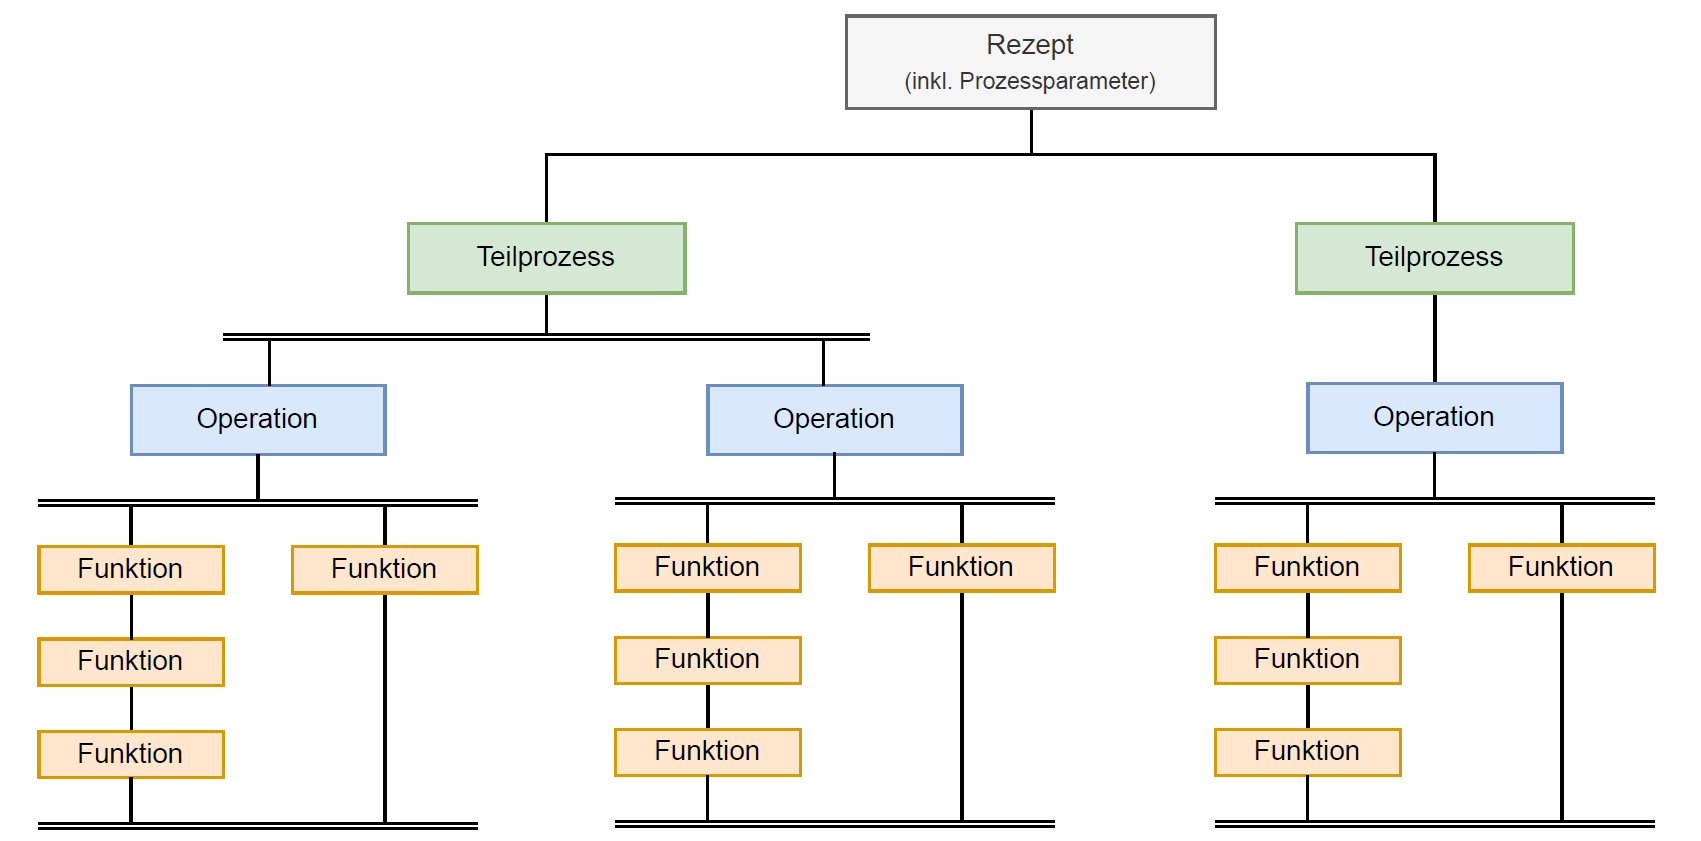
\includegraphics[width=0.8\textwidth]{02_Einfuehrung_in_Thematik/ISA88Struktur}
			\captionsetup{justification=centering}
			\caption{Prozessstruktur von ISA-88}
			\label{fig:Prozessstruktur_ISA88}
		\end{figure}
		
		Das Rezept besteht aus unterschiedlichen Teilprozessen, welche aus Operationen zusammengesetzt sind (\ref{fig:Prozessstruktur_ISA88}). Auf der untersten Stufen befinden sich die Funktionen. Diese stellen die Grundfunktionalitäten der Anlagenkomponenten dar, z.B. das Öffnen und Schliessen eines Ventiles. Alle Prozesse können seriell oder parallel durchgeführt werden. Durch diese Struktur wird der Prozess nicht mit einem fest definierten Ablauf gesteuert, sondern durch die im Rezept definierten Schritte und Parameter. Dies ermöglicht ein flexibles Einsetzen der Anlage und deren Ressourcen. Sofern es die Infrastruktur der Anlage zulässt, kann jedes Rezept gefahren werden. Dies reduziert Stillstandszeiten der Anlage und macht diese effizienter. Dieses Prinzip kann so erweitert werden, dass das System auch selbständig die Anlagenelemente definiert, welche für das Prozessieren der Charge verwendet werden. Hierbei spricht man dann von einer Rezeptur und nicht mehr von einem Rezept. Besteht das System zum Beispiel aus mehreren chemischen Reaktoren, entscheidet die Rezeptur selbständig, welcher der Reaktoren für den Prozess eingesetzt wird. Dies ermöglicht einen noch flexibleren und selbständigeren Prozess.
		
	\vspace{3mm}
	
	\textbf{Frage 1.2:} Wo und wie wird ein chargenorientierter Ansatz eingesetzt \vspace{2mm} 
	\\
		Eine Chargensteuerung nach ANSI/ISA-88 wird hauptsächlich für die Verfahrenstechnik eingesetzt. In der Verfahrenstechnik werden verschiedene Produkte oft auf derselben Anlage hergestellt. Der Einsatz einer Rezeptursteuerung nach ANSI/ISA-88 vereinfacht und standardisiert das Prozessieren von unterschiedlichen Produkten somit erheblich. Für ein neues Produkt muss nur das Rezept angepasst werden, sofern alle Rezepte auf den definierten Funktionen und Operationen aufbauen. 
		
		\begin{figure}[h!]
			\centering
			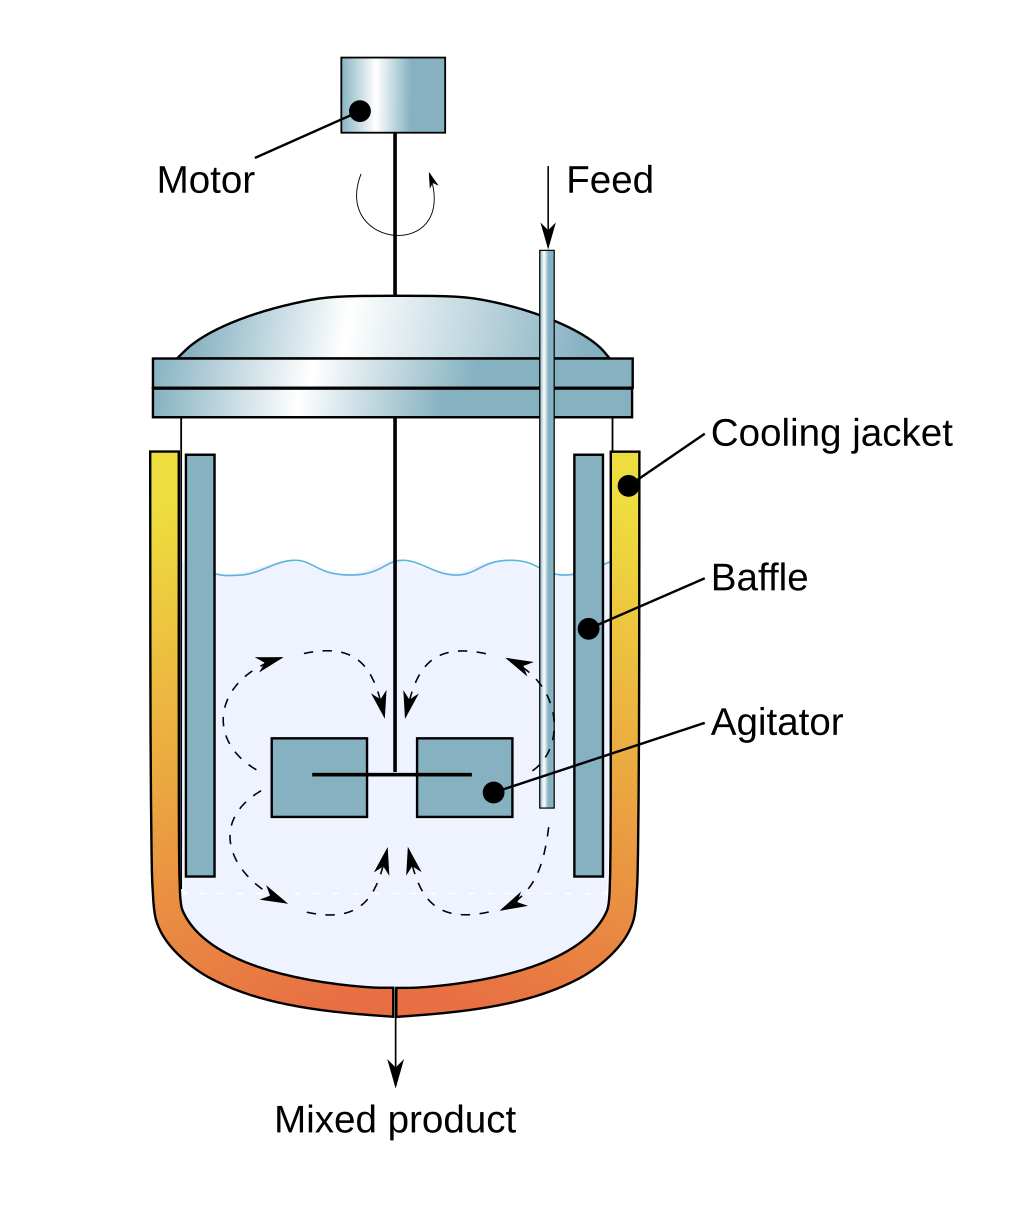
\includegraphics[width=0.3\textwidth]{02_Einfuehrung_in_Thematik/Reaktorbeispiel}
			\captionsetup{justification=centering}
			\caption{Reaktorbeispiel}
			\label{fig:Reaktorbeispiel}
		\end{figure}
		
		Der dargestellte Reaktor (\ref{fig:Reaktorbeispiel}) hat zum Beispiel folgende Funktionen:
		\begin{itemize}
			\item Befüllen
			\item Kühlen
			\item Mischen
			\item Warten
			\item Abfüllen
		\end{itemize}
		\addvspace{5mm} 
		
		Aus diesen Funktionen lassen sich verschiedene Operationen definieren, welche wiederum vom Rezept verwendet werden können, um ein bestimmtes Produkt zu prozessieren. 
		\begin{wrapfigure}{r}{0.5\textwidth}
			\centering
			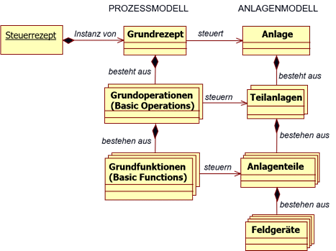
\includegraphics[width=0.5\textwidth]{02_Einfuehrung_in_Thematik/ProzessAnlageModell}
			\captionsetup{justification=centering}
			\caption{Prozess- und Anlagenmodell}
			\label{fig:ProzessAnlageModell}
		\end{wrapfigure}
		Ein zentraler Aspekt für die Flexibilität und Modularität von Chargensteuerungen nach ANSI/ISA-88 ist die Trennung von Prozessmodell und Anlagenmodell (\ref{fig:ProzessAnlageModell}). Das Prozessmodell beinhaltet das Rezept, die Operationen und Funktionen. Die Rezeptlogik ist unabhängig von den spezifischen Elementen, die in der Anlage verwendet wird. Es beschreibt lediglich, was getan werden soll, um das gewünschte Ergebnis zu erzielen, nicht wie oder mit welchen Elementen es durchgeführt wird. Das Anlagenmodel ist für das Ansteuern der Anlagenkomponenten zuständig. Die Trennung von Prozess und Anlage ermöglicht es, dass ein Rezept auf unterschiedlichen Anlagen ausgeführt werden kann. Das Rezept beschreibt, was zu tun ist, unabhängig davon, welche spezifischen Anlagenelemente verfügbar sind.
		
	\vspace{3mm}
	
	\textbf{Frage 1.3:} Wie wird eine chargenorientierte Struktur in TwinCAT umgesetzt \vspace{2mm} 
	\\
		Als Referenz für den Aufbau einer Rezeptursteuerung auf Basis von Codesys dient das Buch «Speicherprogrammierbare Steuerungen in der Industrie 4.0» von Matthias Seitz.
		\\
		Auch in TwinCAT unterscheidet man, wie beschrieben, zwischen dem Prozessmodell und dem Anlagenmodell. Das Prozessmodell beinhaltet das Rezept, die Operationen und die Funktionen. Alle werden mittels Ablaufsprache (AS) umgesetzt. Innerhalb des Anlagenmodells werden die Objektklassen für die verschiedenen Feldgeräte der Anlage definiert. Diese müssen zwingend objektorientiert aufgebaut werden. Die Objektklassen werden in der Anlage instanziiert. Die instanziierten Objekte werden verwendet, um die Schnittstelle zu den Funktionen zu bilden. 
		
		\begin{figure}[h!]
			\centering
			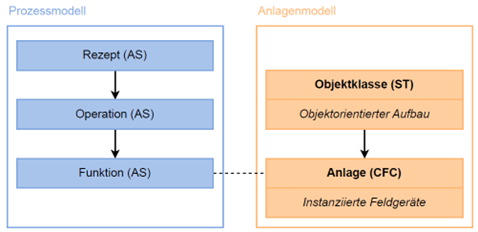
\includegraphics[width=0.7\textwidth]{02_Einfuehrung_in_Thematik/SoftwareStrukturISA88}
			\captionsetup{justification=centering}
			\caption{Softwarestruktur von ISA-88}
			\label{fig:Softwarestruktur_ISA88}
		\end{figure}
		
		Die dargestellte Struktur (\ref{fig:Softwarestruktur_ISA88}) stellt ein stark vereinfachtes Modell dar. Für eine detaillierte Beschreibung der definierten TwinCAT-Struktur, wird auf die Dokumentation des Master-Projekt 2 verwiesen.
		
	\vspace{3mm}
	
	\subsection{Grundlagenfragen für Thematik} \label{Grundlagenfragen für Thematik}
	
	\textbf{Frage 2.1:} Was versteht man unter einem skill-basierten Ansatz \vspace{2mm} 
	\\
		Ein skill-basierter Ansatz basiert auf der Fähigkeit von Maschinen bestimmte Funktionen auszuführen. Der Skill beschreibt eine konkrete Grundfunktion des Systems und stellt die tiefste Abstraktionsebene der Systemfunktion dar. Die Idee hinter dem skill-basierten Ansatz ist, dass Abläufe auf einfache Skills heruntergebrochen werden können. Durch die Verkettung von Skills, mit der Zuweisung von Funktionsparametern, können dann komplexe Funktionalitäten erstellt werden. Das Ziel dieses Ansatzes ist die Vereinfachung der Programmierung eines Systems (z.B. Roboter). In einem traditionellen, nicht-skill-basierten Ansatz würde der gesamte Prozess in einem einzigen, umfassenden Programm geschrieben werden. Das Programm würde alle Schritte in fester Reihenfolge definieren. Änderungen an einem Prozess würden dann oft bedeuten, dass das gesamte Programm geändert werden muss. Dagegen erfordern Änderungen beim skill-basierten Ansatz nur eine Änderung in der Reihenfolge oder Kombination der verwendeten Skills, nicht im gesamten Ablauf.
	\vspace{3mm}
	
	\textbf{Frage 2.2:} Vergleich zwischen einem chargenorientierten und skill-basierten Ansatz \vspace{2mm} 
	\\
		Beide Ansätze besitzen eine vergleichbare Struktur. Die Funktionalitäten eines Systems werden auf der untersten Abstraktionsstufe auf Funktionen bzw. Skills heruntergebrochen. Diese können dann verwendet werden, um komplexere Abläufe zu definieren. Beim skillbasierten Ansatz ist der Einsatz einer Rezeptur mit definierter Chargengrösse weniger sinnvoll. Die Verwendung eines Arbeitsplanes, welcher definierte Schritte vorgibt, eignet sich besser.
		Für den skill-basierten Ansatz werden für den Rahmen dieser Arbeit folgende Begriffe (\ref{fig:Softwarestrukturvergleich}) verwendet, um die verschiedenen Strukturelemente zu beschreiben. 
	
		\begin{figure}[h!]
			\centering
			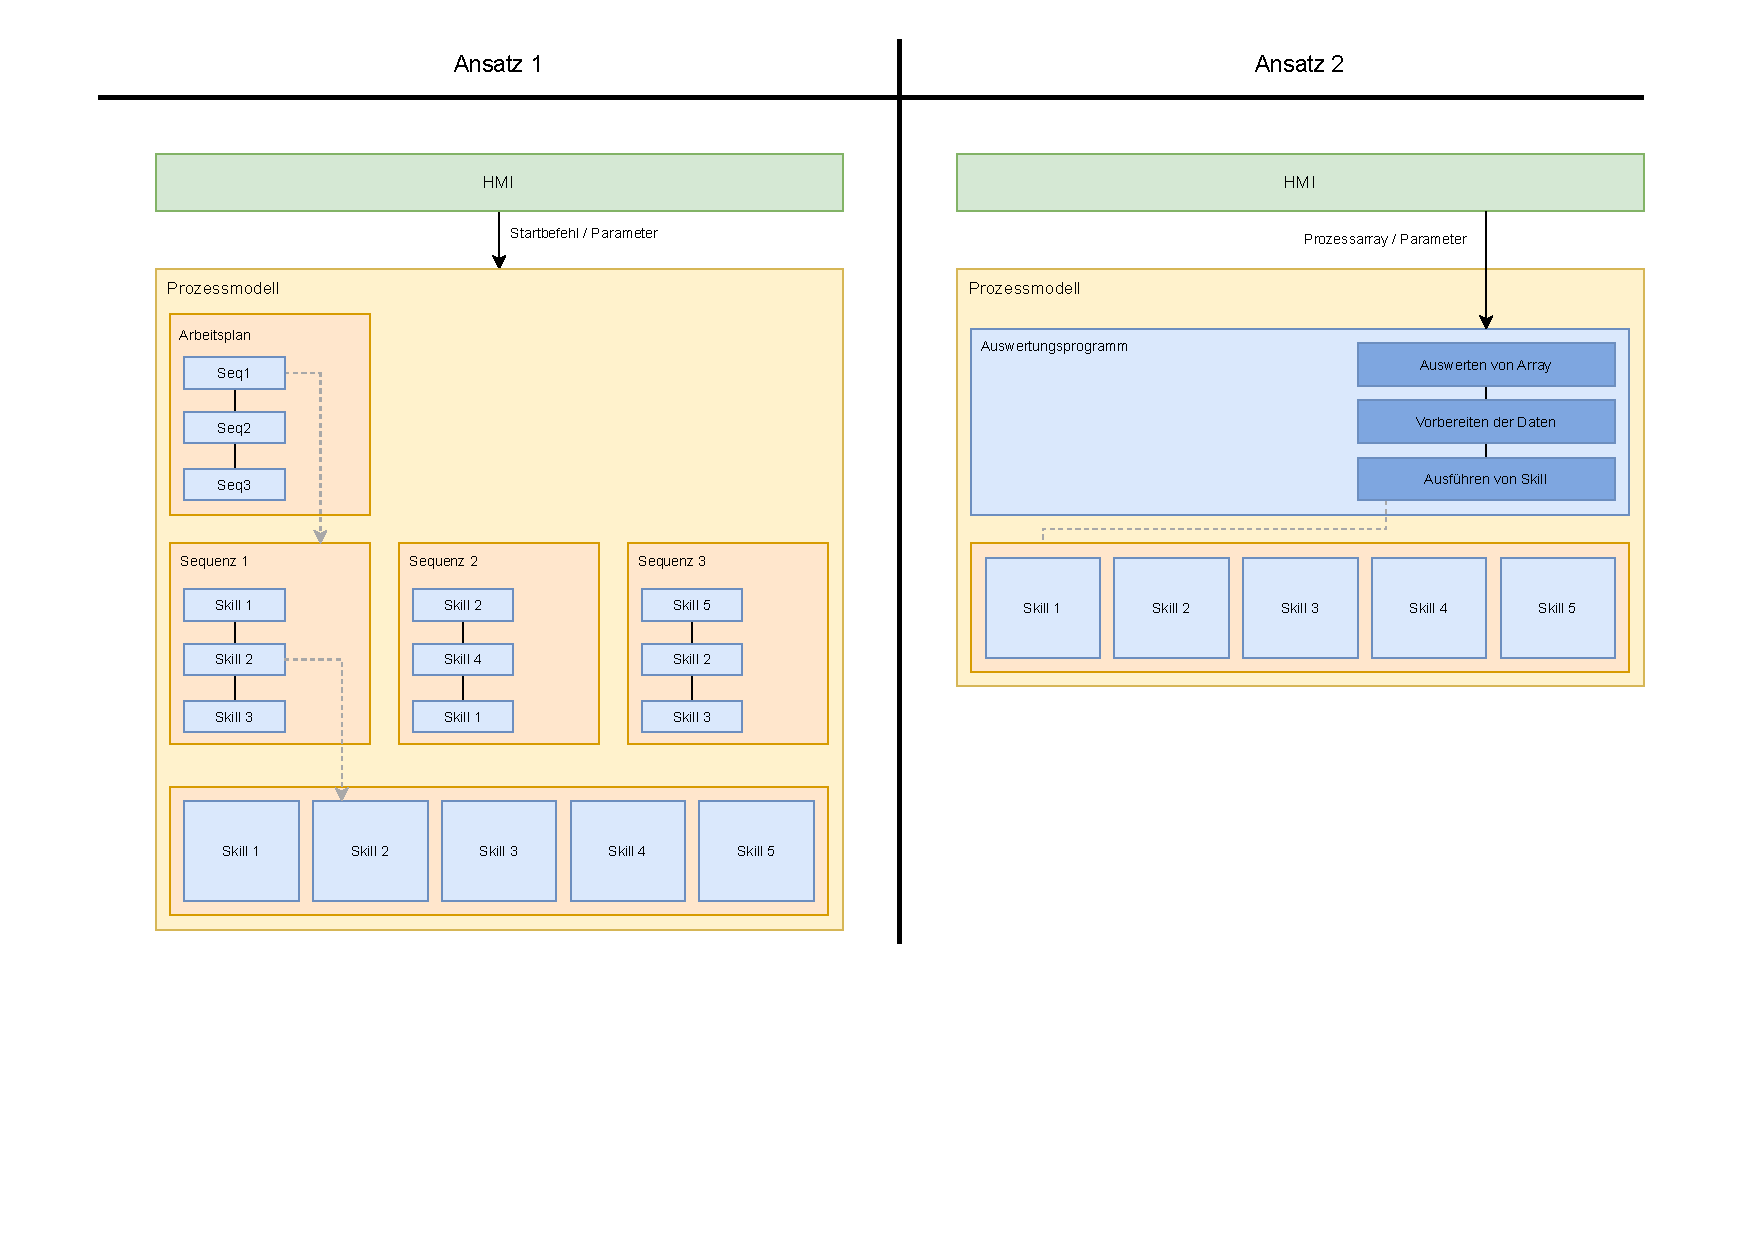
\includegraphics[width=0.4\textwidth]{02_Einfuehrung_in_Thematik/Strukturvergleich}
			\captionsetup{justification=centering}
			\caption{Softwarestrukturvergleich}
			\label{fig:Softwarestrukturvergleich}
		\end{figure}
	
	\vspace{3mm}
	
	\textbf{Frage 2.3:} Was sind die Vorteile eines skill-basierten Ansatzes \vspace{2mm} 
	\\
		Komplizierte Abläufe werden in einfache Teilfunktionen aufgeteilt. Die gesamte Funktionalität des Systems wird entsprechend innerhalb der Skills umgesetzt. Das System kann dadurch einfacher und zugänglicher programmiert werden, da diese modular und flexibel kombiniert und mit entsprechenden Parametern versehen werden können. Dies erhöht auch die Verständlichkeit des Programms für Aussenstehende oder bei nachträglichen Anpassungen. 
		Bei funktionalen Anpassungen werden nur die entsprechenden Skills bearbeitet und nicht das komplette Programm.
		\\
		\begin{wrapfigure}{l}{0.35\textwidth}
			\centering
			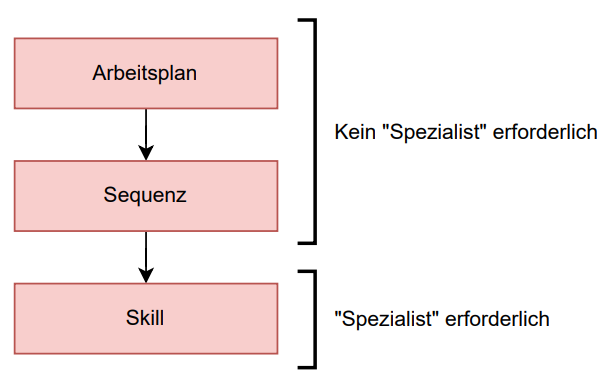
\includegraphics[width=0.35\textwidth]{02_Einfuehrung_in_Thematik/StrukturKompetenzen}
			\captionsetup{justification=centering}
			\caption{Kompetenzaufteilung}
			\label{fig:Kompetenzaufteilung}
		\end{wrapfigure}
		Da die Skills die Schnittstelle zu den Systemkomponenten darstellen, wird nur dort ein fundiertes Wissen über die Programmierung der Komponenten vorausgesetzt. Auf den oberen Stufen (Sequenz / Arbeitsplan) wird kein fundiertes Wissen über die Komponenten benötigt. Die Kompetenzen können bei einem skill-basierten Ansatz somit besser aufgeteilt werden (\ref{fig:Kompetenzaufteilung}). 
		\\
		Ein System, welches mit einem skill-basierten Ansatz programmiert wurde, ist einfach und schnell erweiterbar mit neuen Skills, wenn z.B. neue Produkte auf dem System prozessiert werden sollen. Es ist auch möglich einen Standard für die Schnittstellen der Skills zu definieren. Man beschreibt klar, welche Inputs ein Skill benötigt und welche Outputs dieser liefern muss.
		\\
		\vspace{-7mm}
		\begin{wrapfigure}{r}{0.4\textwidth}
			\centering
			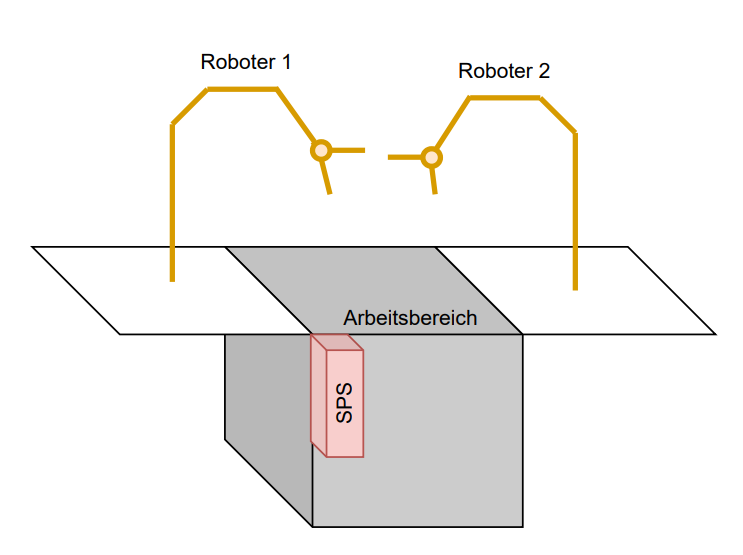
\includegraphics[width=0.4\textwidth]{02_Einfuehrung_in_Thematik/BeispielSystem}
			\captionsetup{justification=centering}
			\caption{Beispielszenario}
			\label{fig:Beispielszenario}
		\end{wrapfigure} \par
		Sequenzen und Arbeitspläne können dadurch anlagenunabhängig aufgebaut werden, da Schnittstellen immer dieselben bleiben. Somit lassen sich Prozess (Sequenzen / Arbeitspläne) bereits definieren, ohne dass die Komponenten im System bekannt sind. Dadurch können auch dynamische Anwendungen realisiert werden.Dies wird anhand einer Beispielsituation erklärt. Ein System besteht aus einem Arbeitsbereich, auf welchem Aufgabe A und B ausgeführt werden soll (\ref{fig:Beispielszenario}).  
		Zur Ausführung dieser Aufgaben besitzt das System zwei Roboter, welche über eine SPS gesteuert werden. Alle Arbeitsprozesse wurden in einzelne Skills aufgeteilt. Durch den anlagenunabhängigen Arbeitsplan kann das System selbst definieren, welcher Roboter Aufgabe A oder B ausführt. Wenn nun Roboter 1 mit Aufgabe A beschäftigt ist, kann Roboter 2 Aufgabe B ausführen oder umgekehrt. Der dynamische Prozess führt zu einer hohen Flexibilität. Roboter 1 und 2 müssen auch nicht vom selben Hersteller kommen. Sofern die Schnittstellen des Skills korrekt definiert wurden, spielt dies für den Prozess keine Rolle. 
	
	\vspace{3mm}
	
	\textbf{Frage 2.4:} Was sind die Herausforderungen eines skill-basierten Ansatzes \vspace{2mm} 
	\\
		Die grösste Herausforderung ist das Herunterbrechen der gesamten Funktionalität einer Roboteranwendung auf Skills. Eine Roboteranwendung kann sehr komplexe Prozesse realisieren, in welchen viele unterschiedliche Aktoren und Sensoren miteinander interagieren. Die umfangreichen Möglichkeiten eines solchen Systems sollen nicht durch die Verwendung von Skills eingeschränkt werden. Falls ein Standard definiert wird, müssen die Systemkomponenten die definierten Schnittstellen zur Verfügung stellen können. Dies wäre ein wichtiger Aspekt einer anlagenunabhängiger Prozessdefinierung auf Stufe der Sequenzen und Arbeitspläne. Zusätzlich soll das Arbeiten mit einem skill-basierten Ansatz nicht aufwändiger werden als das konventionelle Programmieren der Roboteranwendung. 
	\vspace{3mm}
	
	\textbf{Frage 2.5:} Wie wird eine skill-basierte Struktur in TwinCAT umgesetzt \vspace{2mm} 
	\\
		Grundsätzlich kann die Struktur aufgebaut werden wie bei einem chargenorientierten Ansatz. Man hat wieder zwei Modelle, das Prozessmodell und das Anlagemodell. Das Prozessmodell implementiert die Skills, aus welchen die Sequenzen und Arbeitspläne bestehen. Die wohl wichtigsten Elemente der Struktur sind die Objektklassen der Komponenten. Hier wird die Funktionalität der Komponenten, wie z.B. des Roboters, des Greifers aber auch des Vision-Systems programmiert. Diese können dann in der Anlage instanziiert werden. Der Skill greift auf diese instanziierten Objekte zu und führt damit einen definierten Prozess aus. 
	
		\begin{figure}[h!]
			\centering
			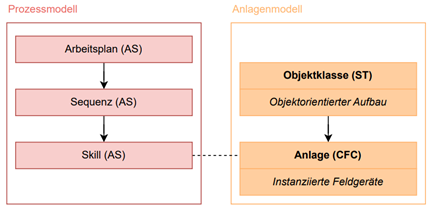
\includegraphics[width=0.7\textwidth]{02_Einfuehrung_in_Thematik/StrukturAngepasst}
			\captionsetup{justification=centering}
			\caption{Angepasste Struktur}
			\label{fig:StrukturAngepasst}
		\end{figure}
		
		Die angegebene Struktur (\ref{fig:StrukturAngepasst}) stellt eine erste Einschätzung dar, welche anhand Erfahrungen des Master-Projekt 2 gemacht wurden. Während der Erarbeitung der Thesis kann sich diese noch verändern. 
	
	\newpage
	
	\subsection{Technische Grundfragen} \label{Technische Grundfragen}
	
	\textbf{Frage 3.1:} Welche Komponenten können im System zum Einsatz kommen \vspace{2mm} 
	\\
		Ein komplettes System kann aus mehreren Aktoren und Sensoren bestehen, welche miteinander interagieren müssen, um einen bestimmten Prozess durchzuführen. Einige mögliche Komponenten werden in der folgenden Liste (\ref{tab:Komponentenliste für Roboter}) aufgezählt.
		
		\begin{table}[h!]
			\centering
			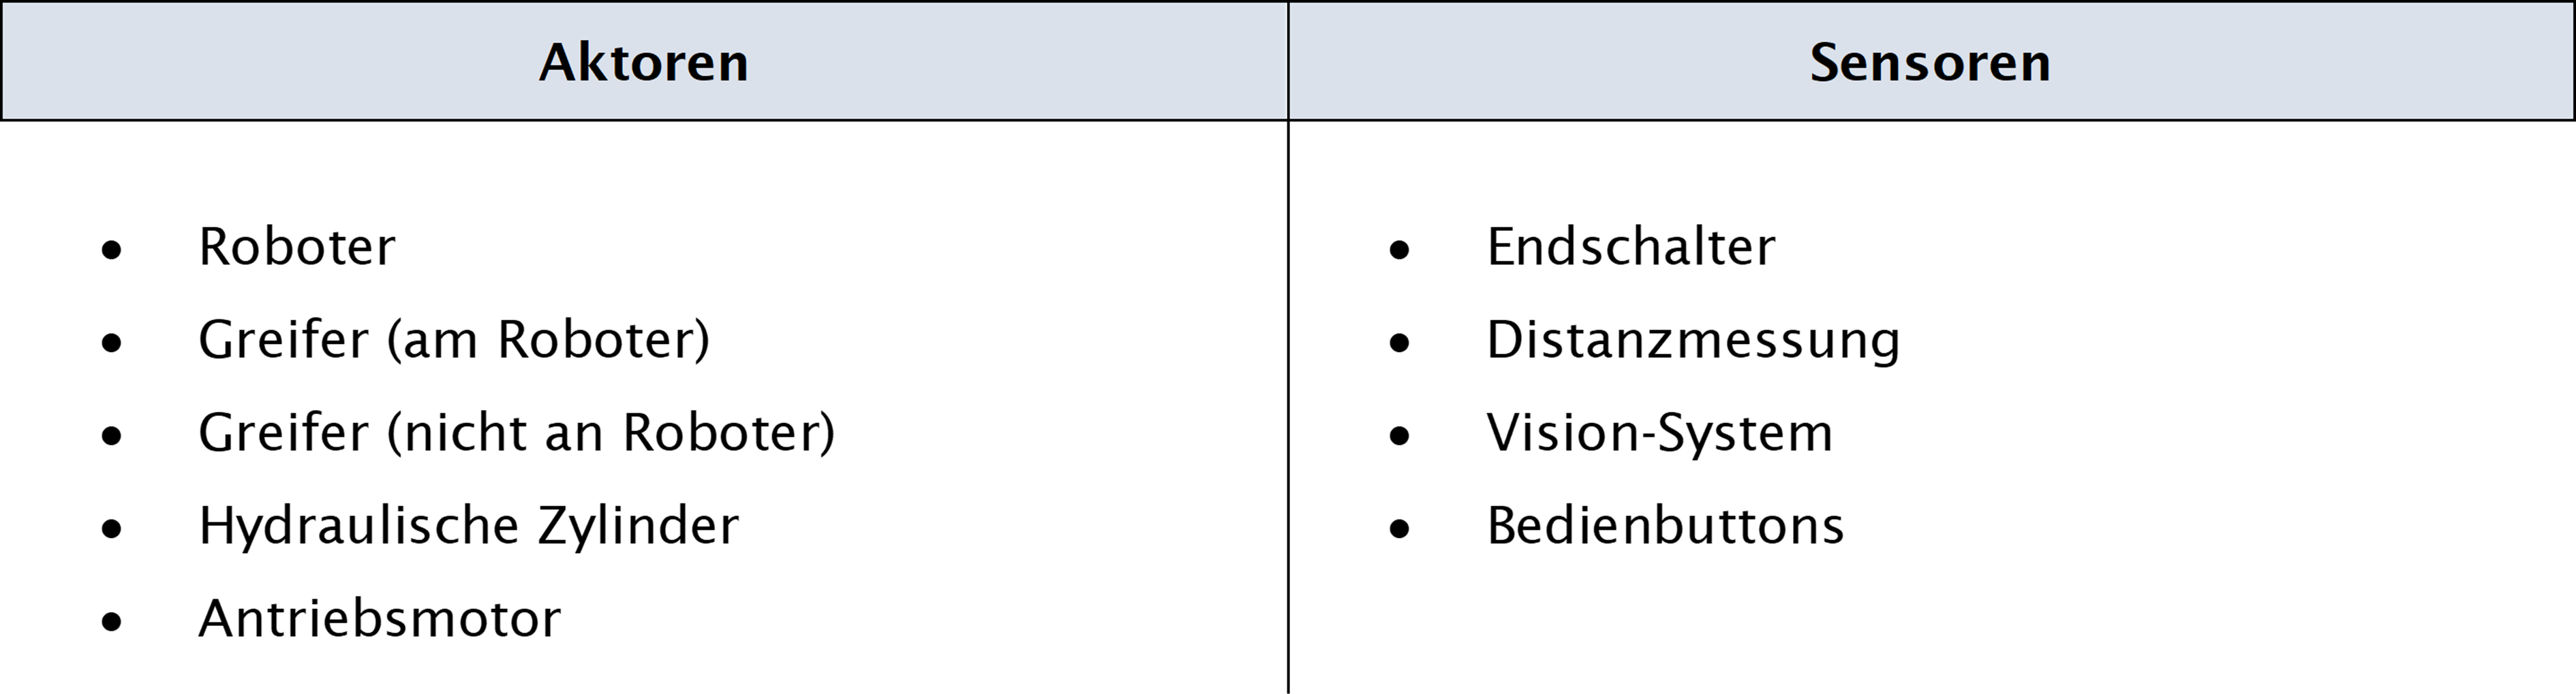
\includegraphics[width=0.8\textwidth]{02_Einfuehrung_in_Thematik/Komponentenliste}
			\captionsetup{justification=centering}
			\caption{Komponenten für Robotersystem}
			\label{tab:Komponentenliste für Roboter}
		\end{table}
		
		Alle Komponenten eines Systems müssen mit der SPS interagieren können und haben einen Einfluss auf den Prozess. Die wohl aufwändigste Schnittstelle ist die SPS-Roboter-Schnittstelle. Fast alle anderen Komponenten können über entsprechende Beckhoff-Klemmen in die SPS integriert werden.
	
	\vspace{3mm}
	
	\textbf{Frage 3.2:} Welche Roboter stehen zur Verfügung \vspace{2mm} 
	\\
		Um eine grosse Bandbreite an Möglichkeiten für das System zu haben, soll für das Projekt ein 6-Achs-Roboter eingesetzt werden. Damit der zeitliche Rahmen der Thesis voll genutzt werden kann, werden Roboter betrachtet, welche im Moment an der BFH, im Bereich der Maschinentechnik, zur Verfügung stehen (\ref{tab:Robotervergleich}). 
		
		\begin{table}[h!]
			\centering
			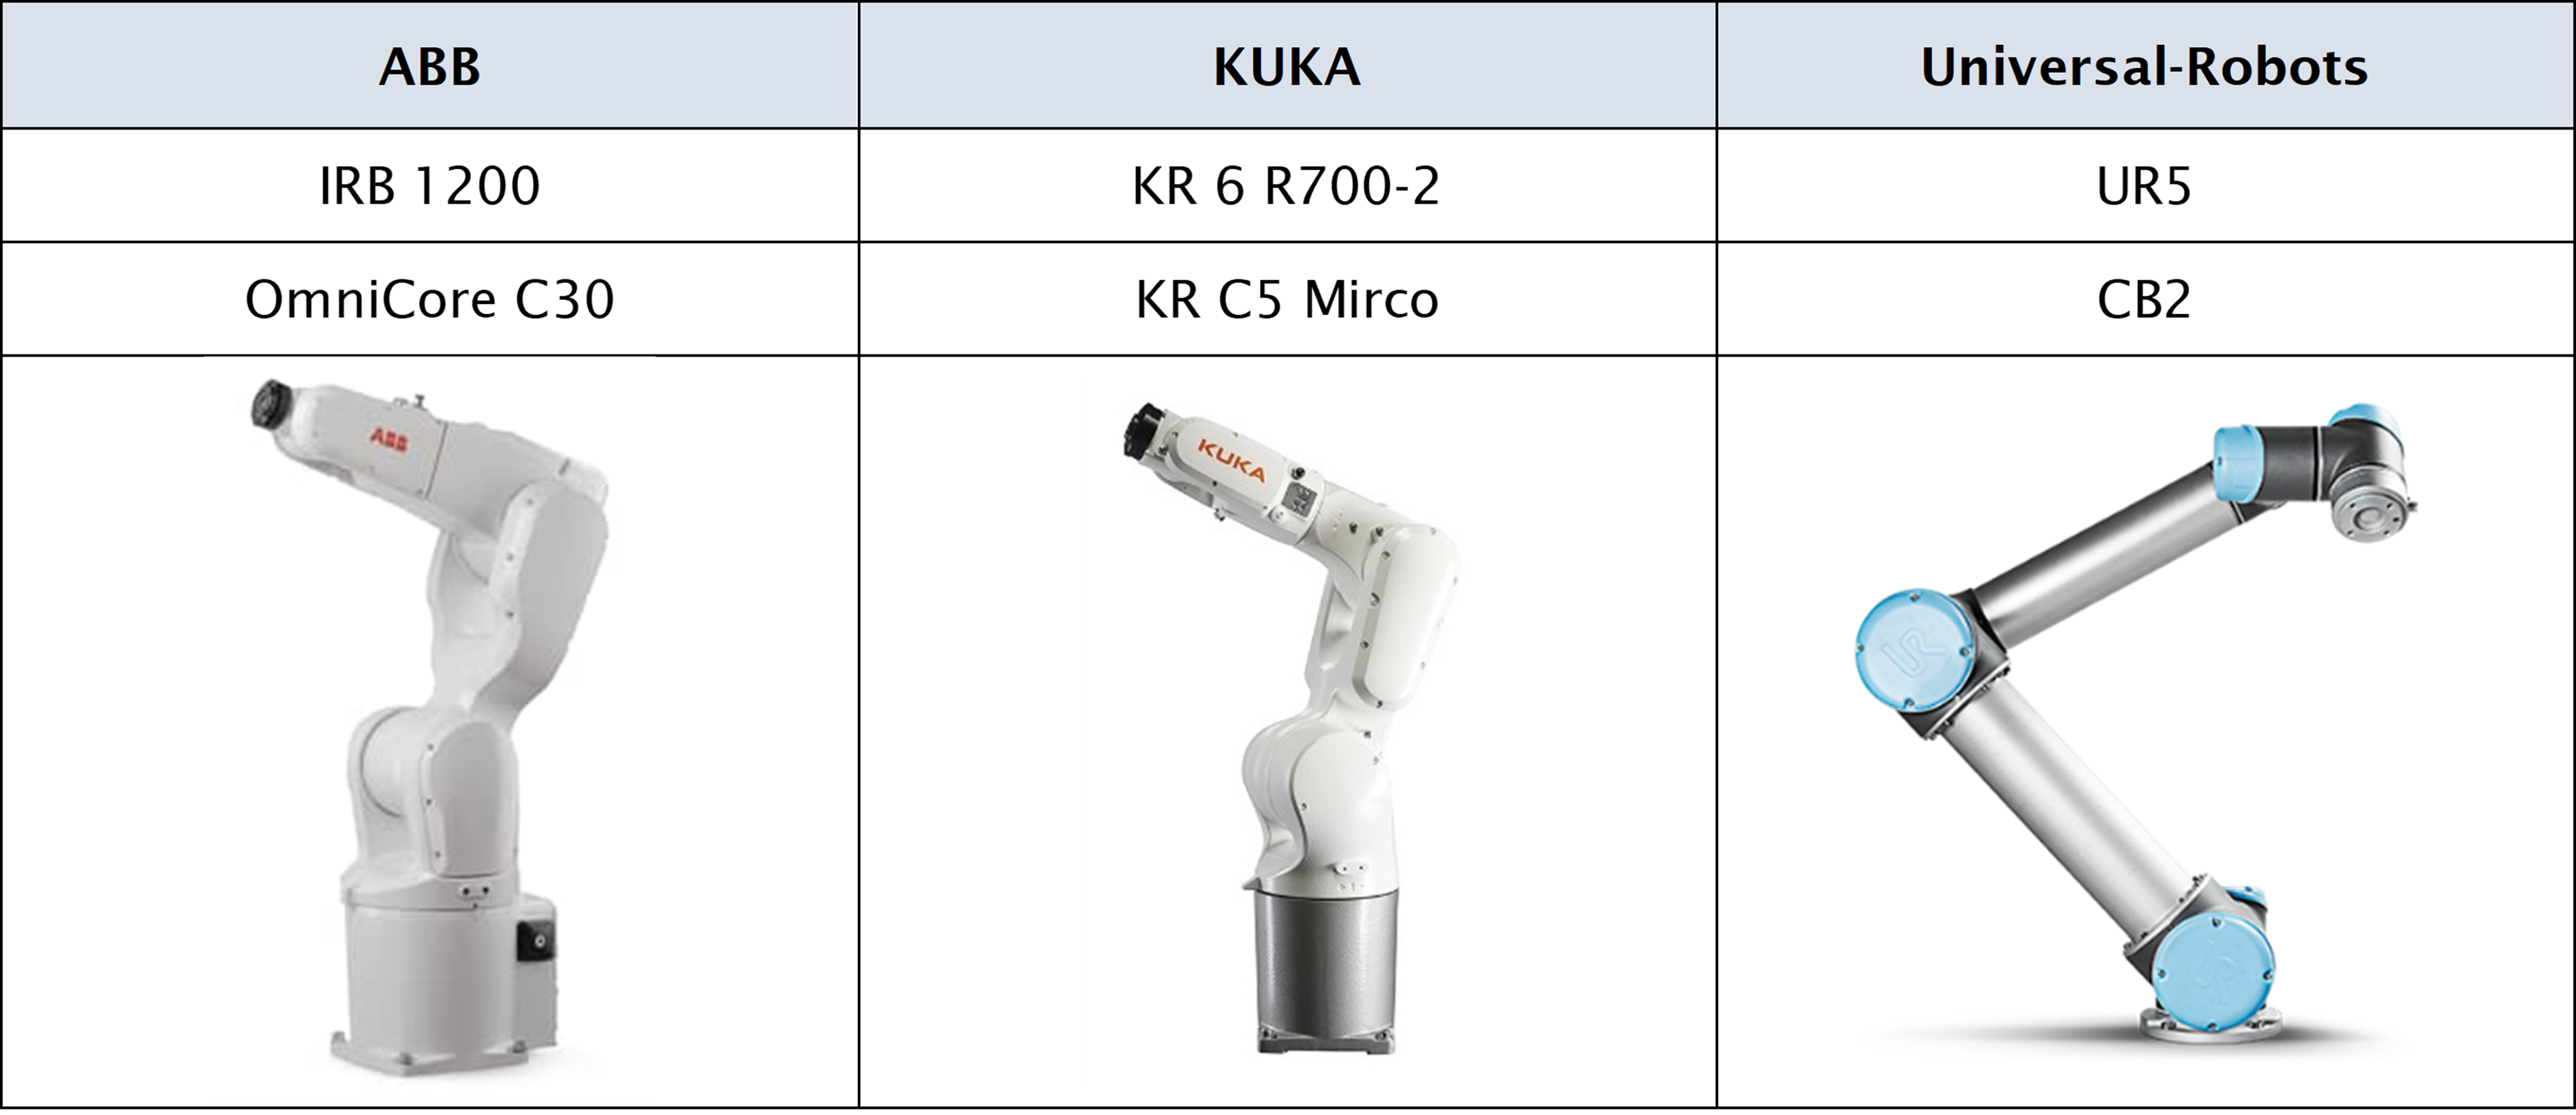
\includegraphics[width=1\textwidth]{02_Einfuehrung_in_Thematik/Robotervergleich}
			\captionsetup{justification=centering}
			\caption{Gegenüberstellung der Roboter}
			\label{tab:Robotervergleich}
		\end{table}
	\vspace{3mm}
	
	\newpage
	
	\textbf{Frage 3.3:} Welche Schnittstellen bieten die Roboter zu einer SPS \vspace{2mm} 
	\\
		Innerhalb dieser Analyse werden die Möglichkeiten aufgelistet, wie die SPS mit dem Roboter verbunden werden könnte. Details über die Kommunikationsschnittstelle oder die benötigten Hersteller-Tools werden bei der Erarbeitung weiter ausgeführt.  
		\vspace{3mm}
		
		ABB (IRB 1200 / OmniCore C30):
		\vspace{2mm}
		\\
		Für die direkte Steuerung eines Roboters kann EGM (Glossar) von ABB verwendet werden.   Mit EGM können Befehle via RAPID-Tasks an den Controller gesendet werden und es können Daten empfangen werden. Die Kommunikation wird über eine UdpUc-Schnittstelle realisiert (\ref{fig:ABB_EGM}). 
		
		\begin{figure}[h!]
			\centering
			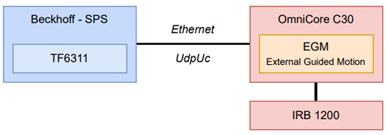
\includegraphics[width=0.5\textwidth]{02_Einfuehrung_in_Thematik/ABB_EGM}
			\captionsetup{justification=centering}
			\caption{ABB-Schnittstelle über EGM}
			\label{fig:ABB_EGM}
		\end{figure}
		
		Es ist auch möglich den Roboter mit OPC UA- oder TCP/IP-Schnittstellen anzusprechen. Hierbei kann jedoch nicht direkt mit dem Roboter kommuniziert werden. Die Verbindung zwischen SPS und Controller wird über RobotStudio von ABB hergestellt. In RobotStudio muss ein Programm laufen, welches die Schnittstellen-Variablen auswertet und interpretiert. Für die OPC-UA-Schnittstelle wird auf der SPS der OPC-UA-Server eingerichtet. RobotStudio dient als Client (\ref{fig:ABB_OPC}).
		
		\begin{figure}[h!]
			\centering
			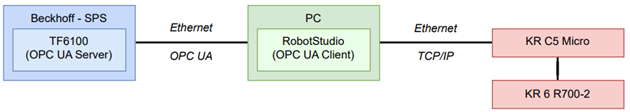
\includegraphics[width=0.9\textwidth]{02_Einfuehrung_in_Thematik/ABB_OPC}
			\caption{ABB-Schnittstelle über OPC}
			\label{fig:ABB_OPC}
		\end{figure}
		\vspace{3mm}
		
		KUKA (KR 6 R700-2 / Kr C5 Mirco):
		\vspace{2mm}
		\\
		Mit «KUKA.PLC mx Automation» bietet KUKA eine standardisierte Schnittstelle zwischen der Robotersteuerung und der SPS. Dies erlaubt es, den Roboter vollständig durch die SPS in Echtzeit zu steuern. Dafür werden Funktionsbausteine zur Verfügung gestellt, welche in der SPS verwendet werden können. Um auf diese zugreifen zu können, muss das Beckhoff-Paket TF5120 (TwinCAT 3 Robotics mxAutomation) installiert werden (\ref{fig:KUKA_mxA}). Eine komplette Liste der Funktionen ist im entsprechenden Beckhoff-Handbuch aufgeführt.
		
		\begin{figure}[h!]
			\centering
			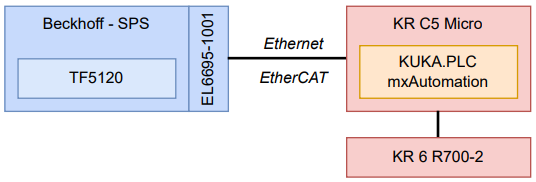
\includegraphics[width=0.5\textwidth]{02_Einfuehrung_in_Thematik/KUKA_MxA}
			\captionsetup{justification=centering}
			\caption{KUKA-Schnittstelle über mxAutomation}
			\label{fig:KUKA_mxA}
		\end{figure}
		
		\newpage
		
		Damit der Kontroller und die SPS miteinander kommunizieren können, wird eine spezielle EtherCAT-Klemme (EL6695-1001) benötigt, welche von KUKA angeboten wird. 
		\\
		Auch eine Schnittstelle über OPC UA ist möglich. Jedoch dient hierbei der Controller als OPC-UA-Server und definiert Kommunikationsvariablen. Die SPS wird als Client eingesetzt. Der Roboter könnte über diese Schnittstelle nur gesteuert werden, wenn auf dem Controller Programme ausgeführt werden, welche die Kommunikationsvariablen auswerten und entsprechende Aktionen auslösen. 
		\vspace{3mm}
		
		Universal-Robots (UR5 / CB2):
		\vspace{2mm}
		\\
		Über eine TCP/IP-Schnittstelle kann die SPS mit dem Controller von Universal Robots kommunizieren. Für eine solche Kommunikationsschnittstelle muss das Beckhoff-Paket TF6310 (TwinCAT 3 TCP/IP) installiert werden (\ref{fig:UR_TCPIP}). Über die von Universal Robots entwickelte Programmiersprache URScript kann der Roboter programmiert werden. URScript ermöglich eine ausführliche Kontrolle über den Roboter.
		
		\begin{figure}[h!]
			\centering
			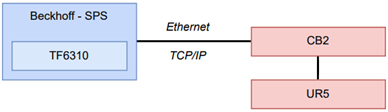
\includegraphics[width=0.6\textwidth]{02_Einfuehrung_in_Thematik/UR5_TCPIP}
			\captionsetup{justification=centering}
			\caption{UR-Schnittstelle über TCP/IP}
			\label{fig:UR_TCPIP}
		\end{figure}
	
	\vspace{3mm}
	
	\newpage
	
	\textbf{Frage 3.4:} Was sind die Anwendungen eines Roboters in der Industrie \vspace{2mm} 
	\\
		Das folgende Mindmap (\ref{fig:Roboteranwendung}) zeigt einen groben Umriss von Anwendungen für einen Roboter in der Industrie. Es wird nicht zwischen kollaborativen und industriellen Roboter unterschieden. 
		
		\begin{figure}[h!]
			\centering
			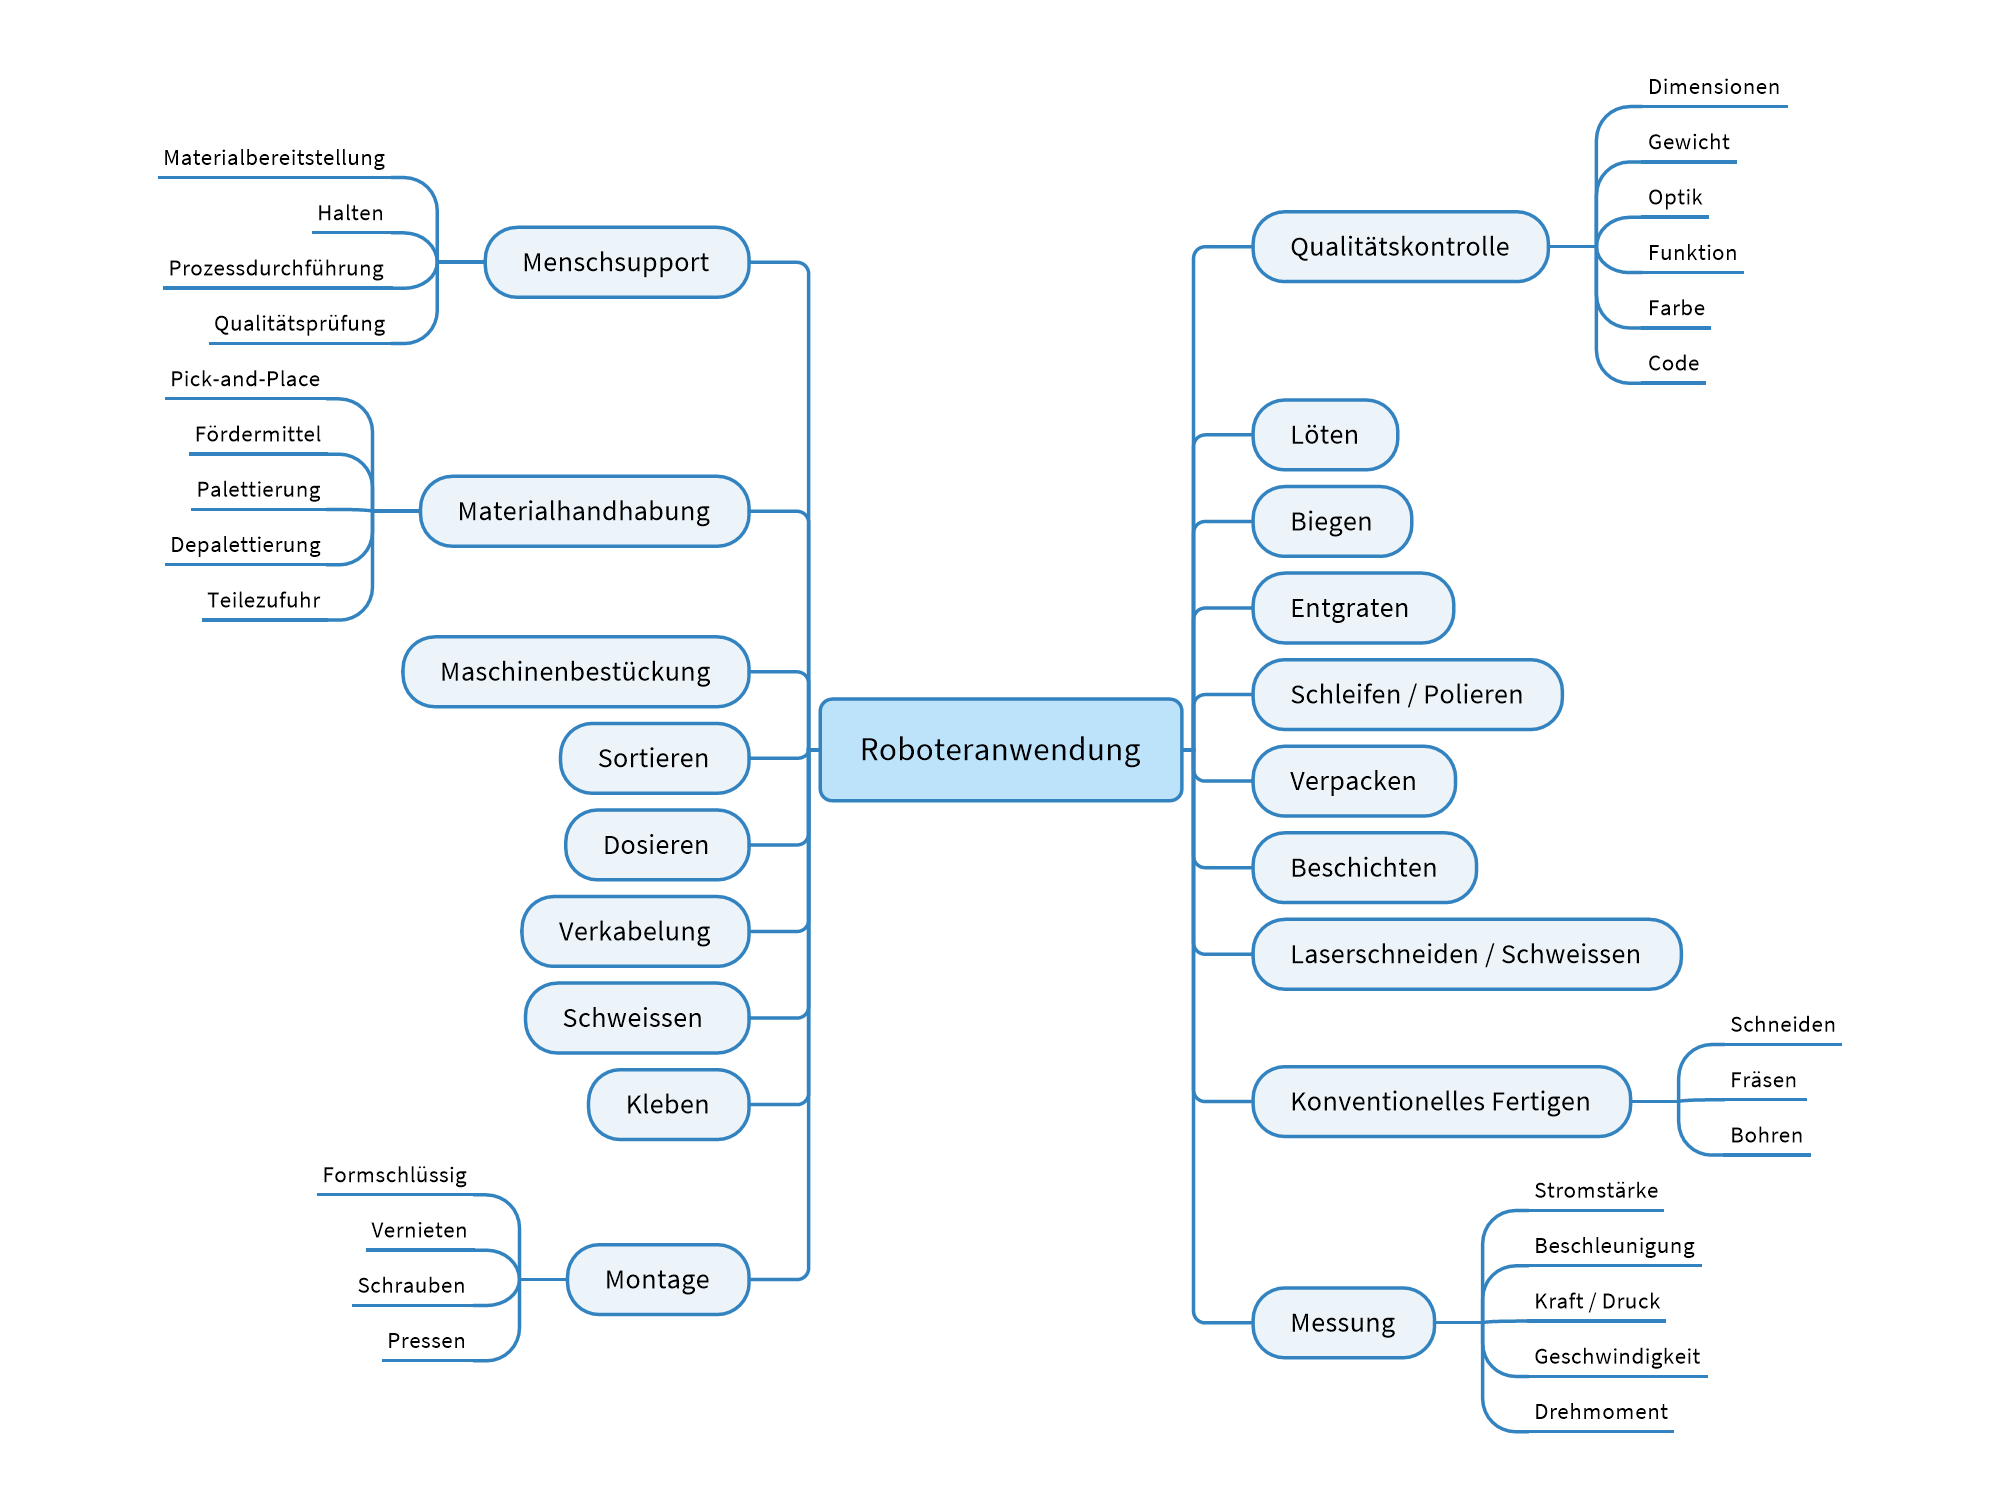
\includegraphics[width=1\textwidth]{02_Einfuehrung_in_Thematik/Roboteranwendung}
			\captionsetup{justification=centering}
			\caption{Roboteranwendung}
			\label{fig:Roboteranwendung}
		\end{figure}
		
		Ein skill-basierter Ansatz eignet sich besonders für Aufgaben, bei denen Anpassungen am Ablauf erforderlich sind, wie beispielsweise bei der Positionierung oder Ausrichtung eines Objekts. Mit diesem Ansatz kann flexibel auf unterschiedliche Situationen reagiert werden. Das traditionelle Teach-In-Verfahren ist hingegen effizienter für Prozesse, die wiederholte und unveränderte Roboterbewegungen erfordern.
		\\
		Während sich ein skill-basierter Ansatz grundsätzlich für viele Anwendungen eignet, entfaltet er seinen Vorteil besonders in Szenarien mit variierenden Bedingungen. Werden hingegen immer dieselben Bauteile verarbeitet, ist das klassische Verfahren oft die bessere Wahl. Bei wechselnden Bauteilen hingegen bietet der skill-basierte Ansatz einen klaren Mehrwert.
		
		
	\vspace{3mm}

	\newpage


\section{Marktanalyse} \label{Marktanalyse}

	\textbf{Frage 1:} Wurden bereits vergleichbare Projekte und Ansätze durchgeführt \vspace{2mm} 
	\\
	
	Referenzprojekt 1:
	\vspace{2mm}
	\\
	\begin{tabularx}{\textwidth}{@{}>{}p{8em} X@{}}
		Rahmen: & 
		MSE-Master-Thesis an der BFH
		\\
		
		Titel: & 
		Skill-basierte Aufgabenplanung für Roboter in Handarbeitsplätzen von Herstellungs-prozessen 
		\\
		
		Beschreibung: & 
		Innerhalb der Master-Thesis wurde für die Firma Ypsomed AG eine spezifische Anwendung mit skill-basierter Aufgabenplanung umgesetzt. Das Ziel dieser Arbeit war eine Roboterlösung zu entwickeln, die einen raschen Einsatz eines Roboters in der Produktion zum Automatisieren verschiedener und wechselnder Aufgaben ermöglicht. Dafür wurden die Teilaufgaben durch parametrierbare Skills umgesetzt, wodurch komplexe Prozessabläufe abgebildet werden konnten.
		
		Das Projekt verwendete einen UR5e-Roboter in Kombination mit einem Greifer und einem Vision-System. Als wichtiges Softwareframework wurde ROS eingesetzt. Jedoch gab es noch weitere Software-Komponenten, welche für das Projekt eingesetzt wurden und miteinander interagiert haben. Das Projekt setzte sich mit Themen wie Lokalisieren der Objekte, das Berechnen des Griffs und das Planen des Roboterablaufs auseinander.
		
		Die Grundfunktionalitäten, welche sich aus der vorgegebenen Anwendung der Firma Ypsomed AG ergaben, wurden als Skills umgesetzt. Die Logik des Skills wurde als Zustandsmaschine aufgebaut. 
		
		Der umgesetzte Prototyp funktionierte für die definierte Anwendung. Einige Funktionalitäten wurden jedoch noch nicht ganz umgesetzt und die Ausführungszeiten des Prozesses sind höher als bei einer händischen Durchführung. 
		\\
		
		Erkenntnisse: & 
		\begin{itemize}
			\item Allgemeine Idee des skill-basierten Ansatzes hat funktioniert
			\item Könnte als Referenz für mögliche Skill-Definition dienen (Parameter/Variablen)
			\item Die umgesetzte Lösung könnte auch mit einer SPS-Schnittstelle betrieben werden
			\item Thematik der Trennung zwischen Prozess und Anlage wurde als zukünftiger Schritt definiert. Im Moment ist die Struktur anlagenspezifisch.
			\item Die umgesetzte Lösung setzt auf viele unterschiedliche Software-Tools mit entsprechenden Schnittstellen
		\end{itemize}
	\end{tabularx}
	
	\newpage
	
	Referenzprojekt 2:
	\vspace{2mm}
	\\
	\begin{tabularx}{\textwidth}{@{}>{}p{8em} X@{}}
		Rahmen: & 
		International Conference on Intelligent Robots and Systems (IROS)
		\\
		
		Titel: & 
		SkiROS2: A skill-based Robot Control Platform for ROS 
		\\
		
		Beschreibung: & 
		Das Dokument beschreibt SkiROS2, welches eine skill-basierte Robotersteuerungsplattform auf Basis von ROS darstellt.  Die Struktur wurde darauf ausgelegt, kleine Batchgrössen, welche komplexe Abläufe benötigen, umzusetzen.  Die Architektur von SkiROS2 besteht aus einem Skill Manager und einem World Model, welche das Kernsystem bilden.
		
		Mit dieser Struktur ist es möglich, mehrere Roboter zu steuern und miteinander zu synchronisieren. Das World Model speichert Instanzen der aktuellen Situation. Es enthält semantische Informationen über Roboter, Objekte und Orte und bietet eine API für das Lesen und Schreiben von Daten. Es kann zur Planung und Parametrisierung von Skills genutzt werden. Jeder Roboter hat einen eigenen Skill Manager, der Skills aus Bibliotheken lädt, diese initialisiert und überwacht. Er übernimmt auch die Ausführung und teilt Aufgaben eindeutig zu.
		
		Alle Skills besitzen die gleiche Struktur. Die Skill-Schnittstelle definiert die benötigten Parameter, wie auch die Pre-, Hold- und Post-Bedingung. Diese werden als Transitionen verwendet, welche den Skill starten, beenden oder abbrechen. Es wird zwischen zwei Skill-Arten unterschieden. Die «primitive» Skills sind Aktionen, welche vom System in der realen Welt ausgeführt werden (z.B. Greifen). Diese haben drei Zustände: «running», «success» und «failure». Die «compound» Skills stellen einen Zusammenschluss von «primitive» oder «compound» Skills dar und sind durch einen Ablauf definiert. 
		
		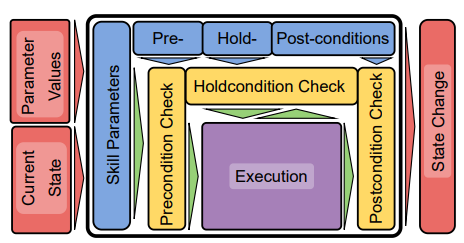
\includegraphics[width=1\linewidth]{02_Einfuehrung_in_Thematik/SkiROS2_Skill}
		\\
		
		Erkenntnisse: & 
		\begin{itemize}
			\item SkiROS2 scheint eine bereits sehr ausgereifte Umsetzung eines skill-basierten Ansatzes zu sein 
			\item Ein Grundwissen über ROS, der allgemeinen Struktur von SkiROS2 und das Programmieren in Python ist erforderlich, um es einsetzen zu können
			\item Ansätze der Strukturierung können als Referenz für Thesis dienen
		\end{itemize}
	\end{tabularx}
	
	\newpage
	
	Referenzprojekt 3:
	\vspace{2mm}
	\\
	\begin{tabularx}{\textwidth}{@{}>{}p{8em} X@{}}
		Rahmen: & 
		Dissertation an der Universität Stuttgart 
		\\
		
		Titel: & 
		Prototypbasiertes Skill-Modell zur Programmierung von Robotern für kraftgeregelte Montageprozess
		\\
		
		Beschreibung: & 
		Die Arbeit zielt darauf ab, den Einsatz von Industrierobotern in Montageanwendungen zu erleichtern, indem ein skill-basierter Ansatz zur Programmierung von kraftgeregelten Montageprozesse entwickelt wurde. 
		
		Innerhalb der Arbeit wurde das komplette System entworfen. Die Skills werden in Bereich Koordination gehandhabt.  
		
		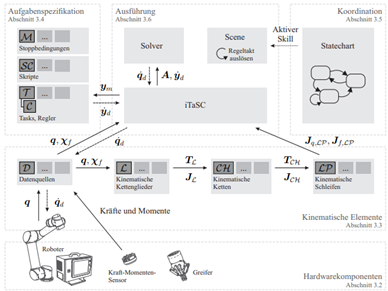
\includegraphics[width=1\linewidth]{02_Einfuehrung_in_Thematik/Disseration_Struktur}
		
		Für das Projekt wurde ein eigenes Skill-Modell entworfen, mit dem Namen «pitasc»
		Das entwickelte Skill-Modell basiert auf drei Grundpfeilern: Abstraktion, Komposition und Vererbung. Hierbei wird eigentlich das Herunterbrechen der Funktionen des Systems auf anlagenunabhängige Parameter beschrieben. 
		
		Die Arbeit wurde für das Fraunhofer-Institut für Produktionstechnik und Automatisierung erstellt. Das Institut bietet den pitasc-Systembaukasten mittlerweile zum Kauf an. 
		\\
		
		Erkenntnisse: & 
		\begin{itemize}
			\item Das pitasc-Skill-Modell könnte für das Projekt spannend sein
			\item Die Thematik der Positions-, Geschwindigkeits- und Kraftregelung kann ein relevanter Punkt werden (z.B. Aufstecken von Klemme auf DIN-Schiene). Die iTaSC-Formulierung könnte dafür hilfreich sein. 
			\item Das entworfene Skill-Modell ist anlagenunabhängig. 
			\item Die Software macht einen sehr komplexen Eindruck, was sich wahrscheinlich in der Anwendung und Bedienung widerspiegelt.
			\item Das beschriebene System beinhaltet kein Vision-System
		\end{itemize}
	\end{tabularx}
	
		\newpage
	
	Referenzprojekt 4:
	\vspace{2mm}
	\\
		\begin{tabularx}{\textwidth}{@{}>{}p{8em} X@{}}
		Rahmen: & 
		Research-Paper des Fraunhofer-Institut für Werkzeugmaschinen und Umformtechnik 
		\\
		
		Titel: & 
		Flexible skill-based control for robot cells in manufacturing
		\\
		
		Beschreibung: & 
		Das Forschungsprojekt stellt die Methode zur Programmierung flexibler, auf Skills basierender Steuerungen für Roboteranwendung vor. Dabei wird stark auf die Vorteile einer solchen Methode eingegangen. Als Hauptvorteil wird die Fähigkeit angegeben, dass der Prozessablauf von Bedienern angepasst und erweitert werden kann, ohne den Steuerungscode zu ändern. Für Entwicklung der Methode wurden vier Anforderungen gestellt: Erweiterbarkeit, Flexible Nutzbarkeit, Konfigurierbarkeit und Wiederverwendbarkeit. Um diese Anforderungen zu erfüllen, wurde die «skill-based control architecture (SBC)» angewendet, welche im Dokument «Evaluating Skill-Based Control Architecture for Flexible Automation Systems» von Kirill Dorofeev und Monika Wenger beschrieben wird. 
		
		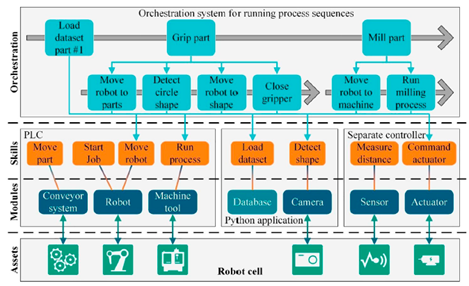
\includegraphics[width=0.8\linewidth]{02_Einfuehrung_in_Thematik/SBC}
		
		Es wird auch darauf hingewiesen, dass es bereits Richtlinien für die Standardisierung von Skills (VDI/VDE/NAMUR 2658) des VDI gibt. Wichtige Begriffe dieser Richtlinie sind PEA (Schnittstellen modularer Prozesseinheiten) und MTP (Module Type Package).
		
		Innerhalb des Projektes wurde ein Prototyp auf Basis von TwinCAT umgesetzt (inkl. HMI). Ein interessanter Aspekt des Systems ist die TwinCAT-Hot-Connect-Funktionalität. Damit können Anlagenkomponenten während des Betriebs entfernt oder hinzugefügt werden. Dies kann für das Wechseln von Greifer während dem Betrieb relevant sein. 
		
		Das Projekt hat gezeigt, dass ein Aufbau mit der SBC-Struktur aufgebaut werden kann und funktioniert. Als weiterführende Arbeiten wurde definiert, dass das benötigte Wissen zur Anwendung von skill-basierten Ansätzen weiter verringert werden muss und das dabei das HMI eine wichtige Rolle spielt. 
		\\
		
		Erkenntnisse: & 
		\begin{itemize}
			\item Das Projekt zeigt, dass eine solche Anwendung auf Basis von TwinCAT umgesetzt werden kann
			\item Das entwickelte HMI kann als Referenz für die Thesis dienen
			\item Die TwinCAT-Hot-Connect-Funktionalität kann für das Projekt relevant sein
			\item Die Richtlinie des VDI kann für das Projekt relevant sein
		\end{itemize}
	\end{tabularx}
	
	\newpage
	
	Die Analyse verdeutlicht, dass bereits zahlreiche Projekte zu diesem Thema durchgeführt wurden, die unterschiedliche Ansätze verfolgen. Diese reichen von reinen Forschungsprojekten bis hin zu Lösungen, die direkt in der Industrie Anwendung finden. Ein skill-basierter Ansatz gewinnt aufgrund neuer und spezifischer Anforderungen der Industrie zunehmend an Bedeutung.
	Die Implementierung eines vollständig skill-basierten Systems umfasst viele unterschiedliche Aspekte, wobei die gewählte Struktur eine zentrale Rolle spielt. Es gibt jedoch zahlreiche Punkte, die für diese Arbeit als Referenz dienen und im Vorfeld geklärt werden müssen. Der Umfang des Themas verdeutlicht, wie wichtig es ist, die Anforderungen an das System präzise zu definieren.
	Keines der analysierten Projekte hat die ISA-88-Norm als Grundlage für seine Struktur verwendet. Die Anwendung dieser Norm auf ein skill-basiertes System stellt daher eine innovative Herangehensweise dar.
	\vspace{3mm}
	
	\textbf{Frage 2:} Was beschreibt die Richtlinie VDI/VDE/NAMUR 2658 \vspace{2mm} 
	\\
	Die Richtlinie beschreibt das Engineering der Automatisierungstechnik modularer Anlagen, insbesondere in der Verfahrenstechnik. Sie behandelt sowohl das Modulengineering als auch das Anlagenengineering. Das Module Type Package (MTP) dient zur Definition und Beschreibung der Schnittstellen und Funktionen der Module, was die Integration in eine Prozessführungsebene ermöglicht. Die Schwerpunkte der Richtlinie umfassen:
	\begin{itemize}
		\item Allgemeines Konzept des modularen Anlagenengineerings
		\item Zustands- und Dienstmodelle modularer Anlagen
		\item Aufbau und Struktur des MTP
		\item Schnittstellen zwischen den Moduldiensten und der Prozessführungsebene (PFE)
		\item Definition des MTP-Manifests und der Kommunikationsschnittstellen (z. B. OPC UA)
		\item Modellierungsvorgaben zur Erstellung des MTP-Manifests und der Kommunikationsbeschreibung.
	\end{itemize}
	Ziel der Richtlinie ist, die Integration von Feldgeräten zu vereinfachen, damit sie effizient mit anderen Systemen zusammenarbeiten. Die Richtlinie stellt sicher, dass die Geräte herstellerunabhängig funktionieren und Daten, wie Mess- oder Diagnosedaten, standardisiert ausgetauscht werden können. Dabei werden nicht nur die Integration in Planungs- und Engineering-Software, sondern auch der Betrieb in Prozessleitsystemen sowie der gesamte Lebenszyklus der Geräte, von der Planung über den Betrieb bis zur Wartung, berücksichtigt. Dadurch können Fehler reduziert und der Aufwand für Inbetriebnahme und Wartung minimiert werden.
	\vspace{3mm}
	
	\newpage
	
	\textbf{Frage 3:} Was ist MTP \vspace{2mm} 
	\\
	MTP steht für Module Type Package und definiert standardisierte Schnittstellen zwischen Anlagenmodulen. Innerhalb eines Systems gibt es verschiedene Module, welche für eine spezielle Prozessfunktion zuständig sind. Dieses Modul wird als Functional Equipment Assembly (FEA) bezeichnet und bildet ein eigenes, geschlossenes System mit Schnittstellen gegen aussen und innen.
	\\
	\begin{figure}[h!]
		\centering
		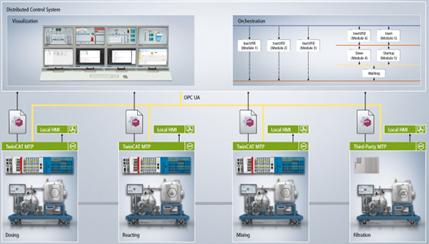
\includegraphics[width=0.8\textwidth]{02_Einfuehrung_in_Thematik/MTP}
		\captionsetup{justification=centering}
		\caption{MTP-Strukur von Beckhoff}
		\label{fig:MTP}
	\end{figure}
	\\
	Ein System besteht aus mindestens einem FEA und bildet das Process Equipment Assembly (PEA). Innerhalb des PEA können FEA entfernt oder hinzugefügt werden. Das MTP definiert eine einfache Konfiguration und Implementation der Anlagenmodule. MTPs definieren die Eigenschaften und Schnittstellen dieser Module. Das Prozessleitsystem liest die MTPs und nutzt diese, um einen Prozessablauf an die Anlagenmodule zu delegieren. Die gesamte Anlage ist dadurch flexibel einsetz- und erweiterbar.
	\\  
	Das MTP-Prinzip wird bis jetzt hauptsächlich in der Verfahrenstechnik eingesetzt. Unternehmen wie Beckhoff, ABB oder Siemens bieten MTP-Pakete für Ihre Systeme an (\ref{fig:MTP}). 
	\\
	Die standardisierte Schnittstellendefinition könnte als Referenz für die Thesis verwendet werden. Jedoch muss die Richtlinie (VDI/VDE/NAMUR 2658) gekauft werden und steht im Moment nicht zur Verfügung. 
	\vspace{3mm}
	
	\textbf{Frage 4:} Was ist der PLCopen-Standard  \vspace{2mm} 
	\\
	Der PLCopen-Standard ist eine internationale Initiative zur Standardisierung von Programmiersprachen und Funktionen einer SPS. Ziel von PLCopen ist es, die Programmierung, Entwicklung und Wartung von Steuerungssystemen zu vereinfachen und zu vereinheitlichen, um die Kompatibilität zwischen verschiedenen SPS-Systemen und Herstellern zu verbessern. Der PLCopen-Standard ergänzt die Norm IEC 61131-3, indem Bibliotheken, Modelle und Richtlinien zur Verfügung gestellt werden, die auf diesen Normen basieren und die Programmierung einer SPS noch effizienter gestalten.
	\\
	Die Richtlinie gibt einen Ansatz vor, wie Funktionsbausteine aufgebaut werden können und funktionieren. Dabei wird zwischen zwei Arten von Funktionsbausteinen unterschieden. Der pegelgesteuerte Funktionsbaustein bleibt aktive, so lange das Triggersignal aktiv ist. Der flankengesteuerte Funktionsbaustein wird bei einer Flanke aktiv und bleibt aktiv. Die Basisdefinition (\ref{fig:PLCopen_FB}) dieser Funktionsbausteine sieht wie folgt aus: 
	
	\newpage
	
	\begin{figure}[h!]
		\centering
		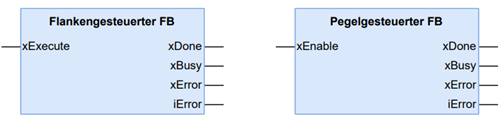
\includegraphics[width=0.8\textwidth]{02_Einfuehrung_in_Thematik/PLCopen_FB}
		\captionsetup{justification=centering}
		\caption{PLCopen-Basisfunktionsblock}
		\label{fig:PLCopen_FB}
	\end{figure}
	
	Diese Basisdefinition kann beliebig erweitert werden, z.B. mit einer Abort-Funktionalität. Das Verhalten der Funktionsbausteine wird anhand des aufgeführten Diagramms (\ref{fig:PLCopen_Ablauf}) erklärt. Die Variable «eState» gibt dabei den momentanen Zustand des Funktionsbausteins als Eigenschaft wieder.
	Der Ansatz der Funktionsbausteindefinition kann für gewisse Aspekte der Thesis relevant sein. Falls Skills als Funktionsbausteine definiert werden, könnte diese Definition helfen, diese übersichtlich und gleich zu strukturieren. 
	
	\begin{figure}[h!]
		\centering
		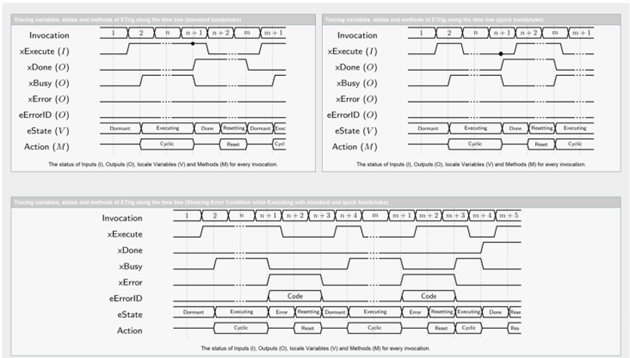
\includegraphics[width=1\textwidth]{02_Einfuehrung_in_Thematik/PLCopen_Ablauf}
		\captionsetup{justification=centering}
		\caption{PLCopen-Basisablauf}
		\label{fig:PLCopen_Ablauf}
	\end{figure}
	
	\newpage
	
	
	